% RLJ main.tex Version 2026.1 (official RLC 2026 template; cover page disabled, style files unmodified)
\documentclass[10pt]{article}

% preprint option: shows author names, removes "under review / RLJ" claims (this is a course report)
\usepackage[preprint]{rlj}

\usepackage{amssymb}
\usepackage{mathtools}
\usepackage{graphicx}
\usepackage{subcaption}
\usepackage{url}
\usepackage{booktabs}
\usepackage{xspace}

\newcommand{\devRandom}{0.0004\,$\pm$\,0.0006}
\newcommand{\lvRandom}{1}
\newcommand{\heRandom}{0}
\newcommand{\helvRandom}{0}
\newcommand{\trRandom}{0.0111\,$\pm$\,0.0080}
\newcommand{\trlvRandom}{4}
\newcommand{\devTba}{0}
\newcommand{\lvTba}{0}
\newcommand{\heTba}{0}
\newcommand{\helvTba}{0}
\newcommand{\trTba}{pending}
\newcommand{\trlvTba}{?}
\newcommand{\devTbb}{0}
\newcommand{\lvTbb}{0}
\newcommand{\heTbb}{pending}
\newcommand{\helvTbb}{?}
\newcommand{\trTbb}{pending}
\newcommand{\trlvTbb}{?}
\newcommand{\devTbc}{0.0044\,$\pm$\,0.0063}
\newcommand{\lvTbc}{3}
\newcommand{\heTbc}{0}
\newcommand{\helvTbc}{0}
\newcommand{\trTbc}{0.0002\,$\pm$\,0.0003}
\newcommand{\trlvTbc}{1}
\newcommand{\devTbcF}{0.0036\,$\pm$\,0.0033}
\newcommand{\lvTbcF}{6}
\newcommand{\heTbcF}{pending}
\newcommand{\helvTbcF}{?}
\newcommand{\trTbcF}{pending}
\newcommand{\trlvTbcF}{?}
\newcommand{\devTca}{0.0004\,$\pm$\,0.0006}
\newcommand{\lvTca}{1}
\newcommand{\heTca}{0}
\newcommand{\helvTca}{0}
\newcommand{\trTca}{pending}
\newcommand{\trlvTca}{?}
\newcommand{\devTcb}{0.0247\,$\pm$\,0.0317}
\newcommand{\lvTcb}{5}
\newcommand{\heTcb}{0.0005\,$\pm$\,0.0006}
\newcommand{\helvTcb}{1}
\newcommand{\trTcb}{0.240\,$\pm$\,0.168}
\newcommand{\trlvTcb}{6}
\newcommand{\devTcc}{0.0003\,$\pm$\,0.0004}
\newcommand{\lvTcc}{1}
\newcommand{\heTcc}{0}
\newcommand{\helvTcc}{0}
\newcommand{\trTcc}{pending}
\newcommand{\trlvTcc}{?}
\newcommand{\devGb}{0.0013\,$\pm$\,0.0010}
\newcommand{\lvGb}{4}
\newcommand{\heGb}{pending}
\newcommand{\helvGb}{?}
\newcommand{\trGb}{pending}
\newcommand{\trlvGb}{?}
\newcommand{\devTda}{0.389\,$\pm$\,0.149}
\newcommand{\lvTda}{9}
\newcommand{\heTda}{pending}
\newcommand{\helvTda}{?}
\newcommand{\trTda}{0.0578\,$\pm$\,0.0469}
\newcommand{\trlvTda}{4}
\newcommand{\devTdb}{0.461\,$\pm$\,0.038}
\newcommand{\lvTdb}{9}
\newcommand{\heTdb}{pending}
\newcommand{\helvTdb}{?}
\newcommand{\trTdb}{pending}
\newcommand{\trlvTdb}{?}
\newcommand{\devTdf}{0.493\,$\pm$\,0.045}
\newcommand{\lvTdf}{9}
\newcommand{\heTdf}{pending}
\newcommand{\helvTdf}{?}
\newcommand{\trTdf}{pending}
\newcommand{\trlvTdf}{?}
\newcommand{\devTdfX}{0.471\,$\pm$\,0.073}
\newcommand{\lvTdfX}{15}
\newcommand{\heTdfX}{pending}
\newcommand{\helvTdfX}{?}
\newcommand{\trTdfX}{0.121\,$\pm$\,0.155}
\newcommand{\trlvTdfX}{7}
\newcommand{\devTdg}{0.494\,$\pm$\,0.045}
\newcommand{\lvTdg}{15}
\newcommand{\heTdg}{pending}
\newcommand{\helvTdg}{?}
\newcommand{\trTdg}{pending}
\newcommand{\trlvTdg}{?}
\newcommand{\devTdh}{0.504\,$\pm$\,0.045}
\newcommand{\lvTdh}{18}
\newcommand{\heTdh}{0.133\,$\pm$\,0.011}
\newcommand{\helvTdh}{22}
\newcommand{\trTdh}{0.0305\,$\pm$\,0.0140}
\newcommand{\trlvTdh}{6}
\newcommand{\devTdi}{0.124\,$\pm$\,0.081}
\newcommand{\lvTdi}{18}
\newcommand{\heTdi}{pending}
\newcommand{\helvTdi}{?}
\newcommand{\trTdi}{pending}
\newcommand{\trlvTdi}{?}
\newcommand{\devTeb}{0.470\,$\pm$\,0.088}
\newcommand{\lvTeb}{26}
\newcommand{\heTeb}{pending}
\newcommand{\helvTeb}{?}
\newcommand{\trTeb}{pending}
\newcommand{\trlvTeb}{?}
\newcommand{\devTec}{0.379\,$\pm$\,0.094}
\newcommand{\lvTec}{28}
\newcommand{\heTec}{pending}
\newcommand{\helvTec}{?}
\newcommand{\trTec}{pending}
\newcommand{\trlvTec}{?}
\newcommand{\devTed}{0.545\,$\pm$\,0.079}
\newcommand{\lvTed}{27}
\newcommand{\heTed}{pending}
\newcommand{\helvTed}{?}
\newcommand{\trTed}{pending}
\newcommand{\trlvTed}{?}
\newcommand{\devTee}{0.568\,$\pm$\,0.063}
\newcommand{\lvTee}{27}
\newcommand{\heTee}{pending}
\newcommand{\helvTee}{?}
\newcommand{\trTee}{pending}
\newcommand{\trlvTee}{?}
\newcommand{\devTef}{0.791\,$\pm$\,0.087}
\newcommand{\lvTef}{27}
\newcommand{\heTef}{0.885\,$\pm$\,0.026}
\newcommand{\helvTef}{34}
\newcommand{\trTef}{0.0203\,$\pm$\,0.0096}
\newcommand{\trlvTef}{11}
\newcommand{\devTefX}{0.667\,$\pm$\,0.222}
\newcommand{\lvTefX}{28}
\newcommand{\heTefX}{0.767\,$\pm$\,0.240}
\newcommand{\helvTefX}{28}
\newcommand{\trTefX}{0.0811\,$\pm$\,0.0498}
\newcommand{\trlvTefX}{12}
\newcommand{\devTeg}{0.791\,$\pm$\,0.087}
\newcommand{\lvTeg}{27}
\newcommand{\heTeg}{pending}
\newcommand{\helvTeg}{?}
\newcommand{\trTeg}{pending}
\newcommand{\trlvTeg}{?}
\newcommand{\devTeh}{0.632\,$\pm$\,0.077}
\newcommand{\lvTeh}{27}
\newcommand{\heTeh}{pending}
\newcommand{\helvTeh}{?}
\newcommand{\trTeh}{pending}
\newcommand{\trlvTeh}{?}

\newcommand{\Tn}[1]{T#1\xspace}
\newcommand{\ours}[1]{\textbf{#1}}

\title{Exploration, not Value Estimation, Limits Learning Agents on ARC-AGI-3}
\setrunningtitle{Exploration, not Value Estimation, Limits Learning Agents on ARC-AGI-3}

\author{[NAME 1]\textsuperscript{1}, [NAME 2]\textsuperscript{1}}
\emails{[NAME 1: student number, student email]; [NAME 2: student number, student email]}
\affiliations{
$^{1}$\textbf{School of Computer Science and Applied Mathematics, University of the Witwatersrand, Johannesburg}\par
Team \emph{Vladmir\_Putin}, COMS4061A/7071A Reinforcement Learning, 2026
}

\keywords{ARC-AGI-3, exploration, DQN, PPO, RND, graph search}
\summary{}

\begin{document}
\maketitle

\begin{abstract}
ARC-AGI-3 asks an agent to discover the rules of unseen games from pixels and to finish their levels in as few actions as a human. We study what limits learning agents here. DQN (with test-time TD learning) and PPO, trained offline on 15 games, each get two stacked improvements, and every improvement is motivated by a measured failure of the previous stage. On a frozen 5-game dev split (500 actions/game, 3 training $\times$ 3 evaluation seeds) both baselines are indistinguishable from random (official score 0.0000 and 0.0004 vs.\ 0.0004). The best learned agent, PPO with random network distillation, reaches 0.025. All learned agents waste their budget re-trying actions that change nothing, and pretrained effect predictors are at chance on unseen games. Replacing learned estimates by explicit per-game online knowledge (a state graph with Thompson-sampled action effects) raises dev score to 0.79, but these gains overfit the dev games: a version with dev score 0.50 scores 0.07 on the hidden Kaggle games. Our leaderboard entry is therefore an attributed fork of Franzen's public LLM agent with three of our own fixes (29.15). We show that single Kaggle scores in this regime are dominated by run-to-run variance and run failures, and we report every run. Code: \url{https://github.com/ThendoNelufule/rl-arc-agi3}.
\end{abstract}

\section{Problem and research question}
ARC-AGI-3 \citep{arcagi3,chollet2019} is a benchmark of turn-based 64$\times$64 games with no instructions: the agent must infer controls, goals and rules by acting, and is scored by how efficiently, relative to humans, it completes levels. The ARC Prize 2026 Kaggle competition \citep{kaggle2026} evaluates agents offline on 110 hidden games within 9 hours. Rewards are sparse (a random agent completes about one level per 7{,}500 actions on our training games) and each game is new, so knowledge transfers only at the level of general behaviour.

\textbf{Research question.} \emph{Can a value-based (DQN) or a policy-gradient (PPO) agent trained offline on public ARC-AGI-3 games learn exploration behaviour that completes levels in unseen games, and what limits it?} \textbf{Contributions.} (i) A Gymnasium adapter and a fixed protocol with a frozen train/dev/held-out split. (ii) Two evidence-driven chains (DQN: novelty, effect masking; PPO: RND, recurrence), all runs reported, with a diagnostic explaining each failure. (iii) A graph explorer built from these diagnostics, including its generalisation failure. (iv) A variance analysis of Kaggle scores for the LLM agent we forked, which we report separately because it is mostly other people's work.

\section{Background and prior work}
\textbf{Scoring.} ARC-AGI-3 uses relative human action efficiency (RHAE): a completed level $l$ with human baseline $b_l$ actions, solved in $a_l$ actions, earns $100\min(1.15,(b_l/a_l)^2)$. Unfinished levels earn 0. A game's score is the level-index-weighted mean ($w_l=l$), and the benchmark score is the mean over games. Late levels therefore dominate, and speed on level~1 is worth little.
\textbf{DQN} \citep{mnih2015} learns $Q_\theta(s,a)$ by minimising the Huber loss to $y=r+\gamma\max_{a'}Q_{\bar\theta}(s',a')$, using replay and a target network. \textbf{PPO} \citep{schulman2017} maximises the clipped surrogate $L^{\text{CLIP}}(\theta)=\mathbb{E}_t[\min(\rho_t\hat A_t,\operatorname{clip}(\rho_t,1{-}\epsilon,1{+}\epsilon)\hat A_t)]$, where $\rho_t=\pi_\theta(a_t|s_t)/\pi_{\theta_{\text{old}}}(a_t|s_t)$. It uses GAE advantages $\hat A_t=\sum_{l}(\gamma\lambda)^l\delta_{t+l}$ with $\delta_t=r_t+\gamma V(s_{t+1})-V(s_t)$ \citep{schulman2016gae}, a value loss and an entropy bonus. Invalid actions are masked in the softmax \citep{huang2022mask}. \textbf{Exploration bonuses:} count-based novelty \citep{bellemare2016} and random network distillation (RND), the prediction error of a trained network against a fixed random one \citep{burda2019}.
\textbf{ARC-AGI-3 agents.} \emph{Stochastic Goose} \citep{smit2025goose}, the preview winner, trains a CNN online to predict which actions change the frame; our effect masking and graph explorer build on this idea, and return-to-frontier search relates to Go-Explore \citep{ecoffet2021}. The 2026 leaders are LLM tool agents. Franzen's Milestone-2 solution \citep{franzen2026m2} patches Tufa Labs' \emph{Duck} harness \citep{tufa2026duck}, the Milestone-1 winner, adding tools, guards and a scheduler over 110 games, with SGLang \citep{zheng2024sglang} serving a 4-bit Qwen3.8-Flash-Next \citep{qwen2026flash}. OpenAI reported that retaining reasoning between turns, plus compaction, tripled their score \citep{openai2026retained}.

\section{MDP formulation}
\label{sec:mdp}
Each game is an episodic POMDP (hidden counters, \S\ref{sec:fail}), which we treat as an MDP over observed frames. Our adapter (\texttt{rl/arc\_gym.py}) defines the following.
\textbf{Observation} $o_t\in\{0..15\}^{1\times64\times64}$: the final animation layer as colour ids, one-hot encoded inside the network. Raw pixels keep the formulation game-agnostic.
\textbf{Actions} \texttt{Discrete(70)}: 0--4 = ACTION1--5, 5 = ACTION7 (undo), and 6--69 = ACTION6 clicks at the centres of an $8\times8$ grid of $8\times8$-pixel cells. A single categorical space with a spatial click head keeps clicks learnable in 400k steps. Illegal actions are no-ops that still cost a step, and \texttt{action\_masks()} exposes legality. Only the graph explorer may also click any pixel (index $70+64y+x$), a change approved after the grid was shown to be its bottleneck (\S\ref{sec:graph}).
\textbf{Reward} $r_t=\max(0,\Delta\,\text{levels\_completed})$, used for training only; we always report the official score.
\textbf{Termination} on WIN or GAME\_OVER, and truncation at 500 actions in training. In evaluation, GAME\_OVER triggers the engine's reset and play continues within the same 500-action budget.
\textbf{What persists.} Between actions: DQN-online weights and its replay of this game, novelty counts, the graph and its statistics, and the LSTM state. Between levels: weights and per-game statistics persist, but the graph is cleared. Between games and evaluation runs: nothing. Weights are restored to the pretrained checkpoint, and each seed gets a fresh Arcade and scorecard.
\textbf{Offline training vs.\ online adaptation.} Learning from other games happens offline on the 15 training games. On an evaluation game, adaptation happens only through the agent's own interaction: test-time TD (DQN-online), recurrent state, or explicit memory (graph). No game-specific code or hidden engine state is used.

\section{Methods}
\label{sec:methods}
All learned agents share one encoder (strided convolutions to an 8$\times$8 map aligned with the click cells; a spatial 1$\times$1-convolution click head and an MLP head for simple actions; 1.19M parameters for DQN), the same 15 training games run as 15 lock-step environments, 400k environment steps, and an episode cap of 500 (full hyperparameters: Table~\ref{tab:hyper}, supplement).

\textbf{DQN chain.} \Tn{10} (baseline, pre-registered): DQN \citep{mnih2015} with masked targets. At evaluation (\texttt{dqn-online}) it takes one TD update per action on the game being played ($\epsilon{=}0.05$), with weights reset to the pretrained ones at the start of every game; the frozen network is reported as variant \Tn{10f}. \Tn{11} adds a count-based novelty bonus $\beta/\sqrt{N(s')}$ ($\beta{=}0.05$, exact frame counts; episodic in training, per game at evaluation). \Tn{12} adds an action-effect head trained with BCE on ``frame changed''. Actions with predicted $p(\text{change})<0.1$ are masked, and at evaluation an exact per-game no-op memory is kept and the head is fine-tuned online.

\textbf{PPO chain.} \Tn{20} (baseline, pre-registered): MaskablePPO \citep{raffin2021sb3,huang2022mask}. \emph{What is learned:} a masked actor $\pi_\theta(a|s)$ and a critic $V_\phi(s)$ on the shared encoder. \emph{When:} after every rollout of $128$ steps $\times$ 15 environments (1{,}920 transitions), GAE ($\gamma{=}0.99$, $\lambda{=}0.95$) advantages are computed and $\theta,\phi$ are updated for 4 epochs of minibatches of 240 on $L^{\text{CLIP}}$ ($\epsilon{=}0.2$) $-\,c_v L^V + 0.01\,\mathcal H[\pi]$. \emph{How it affects decisions:} at evaluation the weights are frozen and actions are \emph{sampled} from the masked policy. An on-policy update inside a 500-action budget would be only a few small batches, so the PPO chain adapts through memory instead. \Tn{21} adds RND \citep{burda2019} with coefficient 0.05 (one combined reward stream). First tests showed the bonus collapsing to $10^{-4}$ within 4k steps, because ARC frames are mostly identical background. Orthogonal target initialisation, per-dimension standardisation of target features, and normalising the bonus by an EMA of the mean error keep it at 0.02--0.05 per step. \Tn{22} makes the \Tn{21} policy recurrent (masked RecurrentPPO, LSTM 256 \citep{hochreiter1997}), with the hidden state reset per game and after GAME\_OVER.

\textbf{Graph explorer} (cross-chain extension, \texttt{rl/policies.py}). It keeps an exact frame-hash state graph per level and never re-tries recorded no-op or deadly $(s,a)$ pairs. It walks a BFS path to the nearest state with untried actions and ranks untried actions by a per-game Beta-Thompson \citep{thompson1933} estimate of their effect, keyed by action or by the colour under the click. \Tn{30} uses no weights at all. \Tn{31} adds $0.3\,\pi(a|s)/\max\pi$ from \Tn{21} as a prior. Later versions (\Tn{32}--\Tn{47}) each fix one failure visible in recordings: step-counter (``ticker'') rows detected online and masked, pruning of actions proven ineffective, visual click equivalence, learned inverse-action pairs (\Tn{37}), object clicks (\Tn{41}--\Tn{44}), and one click per connected component (\Tn{45}).

\textbf{Final leaderboard entry.} Franzen's public Milestone-2 notebook \citep{franzen2026m2} on Tufa Labs' Duck harness \citep{tufa2026duck}: the agent, model, serving and scheduler are theirs. \ours{Our changes} (MOD-F) are three fixes from our own log audit. (1) Reasoning-only replies cut off at the 12{,}288-token output cap are replaced by the harness's existing stub; 13 of 2{,}341 replies in our proxy re-sent $\sim$13k tokens of broken reasoning. (2) A false sentence in the stale-state refusal is corrected and one prompt line states the no-op rules; 92 actions were silently refused after the old advice. (3) The per-game cap is 525 instead of 532 min, because proxy timings projected 32{,}524\,s against a 32{,}400\,s limit. We also tested MOD-1 (two reused public add-ons \citep{heliosli2026,shiiin2026}) and MOD-2 (MOD-1 + Fable facts \citep{leoprovorov2026} + our reinvestment decay).

\section{Experimental setup}
\label{sec:setup}
\textbf{Environments.} We used the 25 public ARC-AGI-3 games in offline mode (\texttt{arc-agi} 0.9.8, \texttt{arcengine} 0.9.3) and no others. They were split once, stratified by type (move/click/mixed), and frozen (\texttt{splits.json}, seed 2026): \emph{train} (15: ar25, cn04, ft09, g50t, m0r0, r11l, re86, s5i5, sb26, sc25, sp80, su15, tr87, vc33, wa30), \emph{dev} (5: dc22, ka59, lf52, lp85, ls20; all decisions), and \emph{held-out} (5: bp35, cd82, sk48, tn36, tu93; evaluated once after development ended). Kaggle uses hidden games. The LLM-agent proxies use all 25 public games, because that agent has no training split.
\textbf{Protocol} (\texttt{rl/evaluate.py}, identical for every agent). The budget is 500 actions per game, counted across deaths, and play stops early only on WIN. Each seed gets a fresh Arcade and scorecard. We log levels, actions, deaths, level-vs-action curves, recordings and the official score for every run. Learned agents use 3 training $\times$ 3 evaluation seeds, and we report the mean $\pm$ SD over training seeds plus all 9 runs. Training-free \Tn{30}/\Tn{35n}/\Tn{45n} use 9 evaluation seeds.
\textbf{Budgets, stopping, checkpoints.} A fixed 400k steps, with no early stopping, and the final checkpoint is used. Training seed 0 for Kaggle, the baselines, and the evaluation-time convention were all pre-registered before any result.
\textbf{Hardware.} Training ran on Kaggle T4 GPUs (4 vCPU Xeon 2.0\,GHz) and evaluation on Kaggle CPU kernels (1 thread per job; after a laptop out-of-memory crash, three agents were re-run there with identical results). Python 3.13.15, PyTorch 2.11.0, NumPy 2.1.3, Gymnasium 1.2.0 \citep{towers2024gymnasium}, SB3/sb3-contrib 2.9.0; the submission image uses Python 3.12.13 and PyTorch 2.10.0 (CPU). \textbf{Cost} (Table~\ref{tab:compute}, supplement). \emph{Training:} 0.30--0.50 T4-hours per seed for DQN versions, 0.37--0.46 for PPO and 0.94 for PPO-LSTM; 10.45 T4-hours in total over 21 runs. \emph{Evaluation} (3 seeds $\times$ 5 games $\times$ 500 actions, 1 CPU thread): 1{,}066--1{,}350\,s for DQN-online (test-time TD), 68--110\,s for PPO, and 89--123\,s for the graph explorer, which needs no training beyond the \Tn{21} prior.


\section{Results}
\label{sec:results}
\begin{figure}[t]
\centering
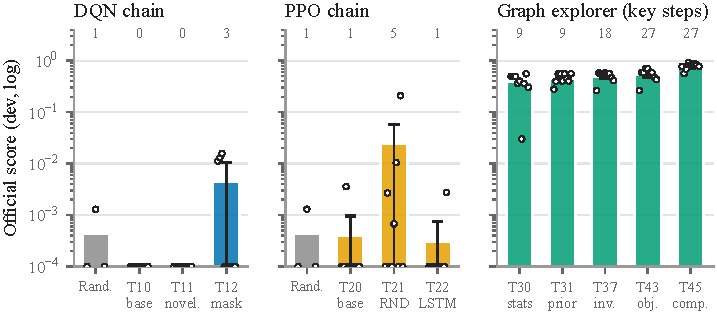
\includegraphics[width=\textwidth]{figs/ladder.pdf}
\caption{Official dev score (log scale; numbers = levels over all runs). Bars: mean over 3 training seeds, error bar: SD over training seeds; dots: all 9 runs, zeros at $10^{-4}$. Random/\Tn{30}: no training (3/9 eval seeds). Colour = agent family throughout.}
\label{fig:ladder}
\end{figure}

\begin{table}[t]
\centering\scriptsize\setlength{\tabcolsep}{3pt}
\caption{Master results (official score). Dev: mean\,$\pm$\,SD over training seeds; Lv: levels over all dev runs (of 342; random of 114); level~1: solving runs @ actions taken. No agent finished a game, so every run used all 500 actions. Train/held-out: means over 3--9 eval seeds (learned: training seed 0); --: not run. Kaggle: public LB, training seed 0. $^\dagger$Starter random agent.}
\label{tab:master}
\resizebox{\textwidth}{!}{\begin{tabular}{@{}llrrlrrr@{}}
\toprule
Ver. & Change & Dev score & Lv & Level~1 on dev: runs @ actions & Train & Held-out & Kaggle \\
\midrule
Rand. &  & 0.0004\,$\pm$\,0.0006 & 1 & lp85 1/3 @352 & 0.0111 & 0 & 0.02$^\dagger$ \\
\midrule
T10 & DQN & 0 & 0 & -- & -- & 0 & 0.00 \\
T11 & +novelty & 0 & 0 & -- & -- & -- & 0.00 \\
T12 & +effect mask & 0.0044\,$\pm$\,0.0063 & 3 & lp85 3/9 @101--120 & 0.0002 & 0 & 0.00 \\
\midrule
T20 & PPO & 0.0004\,$\pm$\,0.0006 & 1 & lp85 1/9 @212 & -- & 0 & 0.00 \\
T21 & +RND & 0.0247\,$\pm$\,0.0317 & 5 & lp85 4/9 @124--489; ls20 1/9 @41 & 0.240 & 0.0005 & 0.05 \\
T22 & +LSTM & 0.0003\,$\pm$\,0.0004 & 1 & lp85 1/9 @241 & -- & 0 & -- \\
\midrule
T30 & graph+online stats & 0.389\,$\pm$\,0.149 & 9 & lp85 9/9 @16--72 & 0.0578 & -- & -- \\
T31 & +PPO prior & 0.461\,$\pm$\,0.038 & 9 & lp85 9/9 @12--24 & -- & -- & -- \\
T37 & +inverse actions & 0.504\,$\pm$\,0.045 & 18 & lp85 9/9 @15--25; ls20 9/9 @128--287 & 0.0305 & 0.133 & 0.07 \\
T43 & objects as fallback & 0.545\,$\pm$\,0.079 & 27 & lf52 9/9 @52--349; lp85 9/9 @15--25; ls20 9/9 @128--287 & -- & -- & -- \\
T45 & component clicks & 0.791\,$\pm$\,0.087 & 27 & lf52 9/9 @24--56; lp85 9/9 @14--30; ls20 9/9 @128--287 & 0.0203 & 0.885 & -- \\
T45n & no prior & 0.667\,$\pm$\,0.222 & 28 & lf52 9/9 @23--59; lp85 9/9 @11--33; ls20 8/9 @128--374 & 0.0811 & 0.767 & -- \\
\bottomrule
\end{tabular}
}
\end{table}

\subsection{Baselines: both learners are indistinguishable from random}
\label{sec:baselines}
Random scores 0.0004 on dev (1 level in 3 runs), \Tn{10} and its frozen variant score 0 (0 levels in 9), and \Tn{20} scores 0.0004 (1 in 9). On Kaggle all three score 0.00--0.02 (Table~\ref{tab:master}). Fig.~\ref{fig:training} explains why. In 400k steps the DQN seeds see only 7/4/8 rewards, the Q-values stay flat ($\approx$0.05, loss $\approx10^{-5}$), and greedy selection degenerates: the frozen \Tn{10f} spends 77--93\% of its actions on one action, and with test-time TD the top-action share is still 0.34--0.40 (random: 0.08). PPO does not collapse, but with 3--5 rewards per seed its entropy only falls from 3.49 to $\approx$3.0 nats, leaving near-uniform behaviour. \emph{The limit is the missing learning signal, not capacity.}

\begin{figure}[t]
\centering
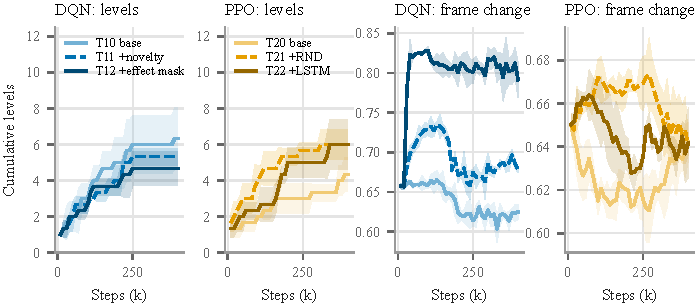
\includegraphics[width=\textwidth]{figs/training.pdf}
\caption{Training curves, mean $\pm$ SD over 3 training seeds. Left: cumulative level completions (all rewards seen in 400k steps on 15 games). Right: fraction of actions that change the frame. Effect masking (\Tn{12}) raises the frame-change rate from 0.61 to 0.77--0.82 without increasing reward, and no version gets more than 8 rewards per run.}
\label{fig:training}
\end{figure}

\subsection{Improvements: each stage removes one diagnosed failure}
\label{sec:improve}
Each step below runs limitation $\to$ hypothesis $\to$ intervention $\to$ result.
\textbf{\Tn{11} (novelty).} \emph{Limitation:} no learning signal (\Tn{10}). \emph{Hypothesis:} a dense count bonus breaks the collapse. \emph{Result:} the training frame-change rate rises from 0.61 to 0.67, but dev score stays 0 and the collapse is slightly worse (top action 0.50--0.58). New diagnostic: 27--33\% of \emph{all} actions repeat an $(s,a)$ already seen to change nothing (random: 7\%), which the bonus penalises only slowly through TD.
\textbf{\Tn{12} (effect masking).} \emph{Hypothesis:} predicting and masking ineffective actions removes this waste. \emph{Result:} repeated known no-ops fall to 0.169/0.012/0.042, and \Tn{12} is the first DQN version to complete levels on dev (0.0044\,$\pm$\,0.0063, 3 levels, all lp85; frozen variant 0.0036, 6 levels). However, the pretrained effect head has a within-game AUC of 0.42--0.58 on unseen dev games: \emph{chance}. A PPO-trained effect model (\Tn{23}) is also at chance (0.39--0.54, excluding the trivial ls20). The gain comes from the exact per-game memory, not from pretraining.
\textbf{\Tn{21} (RND).} \emph{Limitation:} PPO barely moves from uniform. \emph{Hypothesis:} a learned novelty signal that generalises across near-identical frames gives a dense gradient. \emph{Result:} the largest learned-agent gain, 0.0247\,$\pm$\,0.0317 with 5 levels (lp85 4/9, ls20 1/9). The variance is large: one ls20 solve in 41 actions scores 0.2085 by itself and dominates the mean, because efficiency is squared.
\textbf{\Tn{22} (LSTM).} \emph{Limitation:} the memoryless \Tn{21} still re-tries known no-ops (8--10\% of actions). \emph{Hypothesis:} recurrence lets the policy remember failed actions. \emph{Result:} \textbf{failure}, 0.0003 with 1 level. Repeated no-ops are not reduced (0.059--0.138), and training cost doubles (0.94\,h/seed). 400k steps on 15 games do not teach an LSTM to ``not repeat what failed''.
\emph{Established:} for both algorithms the constraint is exploration inside an unseen game. The knowledge that helps (what does nothing, where the agent has been) is game-specific and must be explicit and acquired online.

\subsection{Graph explorer and ablations}
\label{sec:graph}
\begin{figure}[t]
\centering
\begin{minipage}[t]{0.6\textwidth}\vspace{0pt}
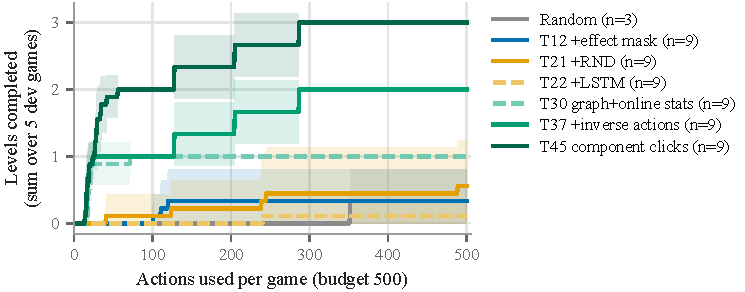
\includegraphics[width=\textwidth]{figs/levels_actions.pdf}
\end{minipage}\hfill
\begin{minipage}[t]{0.38\textwidth}\vspace{2pt}
\caption{Levels completed on the 5 dev games vs.\ actions used (mean $\pm$ SD over runs). Learned agents complete levels late and rarely. The graph explorer solves lp85 level~1 in 14--30 actions (human baseline 17) and lf52 level~1 in 24--56 (human 32), but no version finishes a game or reaches level~2 on lp85/ls20 within 500 actions.}
\label{fig:levels}
\end{minipage}
\end{figure}
The graph explorer applies these findings directly. With online statistics alone, \Tn{30} scores 0.389 and solves lp85 level~1 in every run. The \Tn{21} policy as a prior gives \Tn{31} 0.461\,$\pm$\,0.038. Each later step was diagnosed from recordings (supplement, Fig.~\ref{fig:prog}). Masking the step-counter (``ticker'') rows restores state identity, because the bar otherwise makes every frame new (\Tn{32}). Inverse action pairs learned online cut navigation cost: ls20 level~1 is solved in 9/9 runs after 128--287 actions instead of 6/9 after 367--473 (\Tn{37}, 0.504, 18 levels). Every remaining failure traced to the 8$\times$8 click grid: with 1000 or 2000 actions \Tn{37} reaches the same 18 levels, because its reachable frontier is exhausted. With pixel clicks, objects as a fallback tier (\Tn{43}, 0.545, 27 levels) and one click per connected component (\Tn{45}, \textbf{0.791\,$\pm$\,0.087}; lf52 level~1 at human speed) gave the largest gain. Some variants failed: patch-keyed statistics (\Tn{38}, 0.124) slowed lp85, and a size prior (\Tn{47}, 0.632) traded lp85 for lf52.
\textbf{PPO prior ablation.} Without the prior, \Tn{35n} scores 0.471 with 15 levels, vs.\ \Tn{35} 0.493 with 9. The prior speeds up lp85 clicks but biases movement and prevents ls20 solves, and applying it to clicks only (\Tn{36}: 0.494, 15 levels) keeps both gains. For the final design, \Tn{45n} scores 0.667 vs.\ \Tn{45} 0.791. The difference comes from ls20 (8/9 vs.\ 9/9 solves, up to 374 vs.\ 287 actions) and is within one SD of \Tn{45n}'s runs (0.222). The learned prior contributes a small, game-dependent ordering bias. The explorer's structure, not learning, produces the gain.

\subsection{Generalisation: dev gains do not transfer to hidden games}
\label{sec:gen}
\begin{figure}[t]
\centering
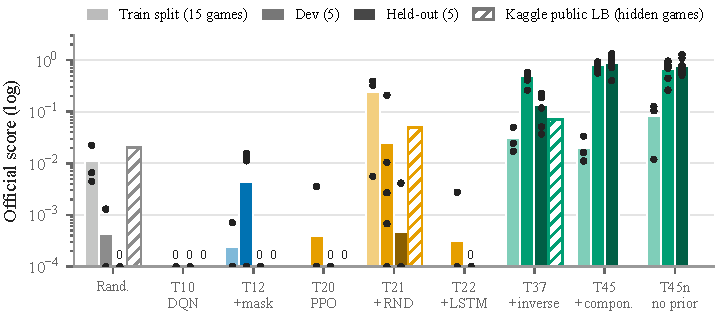
\includegraphics[width=\textwidth]{figs/generalisation.pdf}
\caption{Official score by evaluation set (log scale; dots = runs). Train: training seed 0 (for learned agents, their own training games). Held-out: evaluated once, after development. Kaggle: one public-LB run on hidden games.}
\label{fig:gen}
\end{figure}
The graph explorer's dev score was optimised over 18 versions on 5 games, and it shrinks off dev. On the 15 training games, which it never saw, the no-prior logic scores 0.121 (\Tn{35n}; dev 0.471) and 0.081 (\Tn{45n}; dev 0.667). On Kaggle, \Tn{37} (dev 0.504) scores \textbf{0.07}. Held-out: \Tn{45} \heTef{} and \Tn{37} \heTdh{} (random \heRandom{}). \emph{Dev overfitting is the main lesson of the graph track.} Five dev games with one or two solvable first levels rewarded orderings fitted to them, and the late levels that RHAE weights most were never reached.

\subsection{Final leaderboard entry and the variance of Kaggle scores}
\label{sec:final}
\begin{figure}[t]
\centering
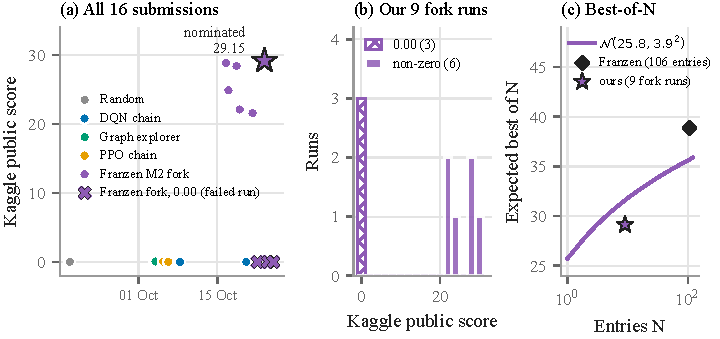
\includegraphics[width=\textwidth]{figs/kaggle.pdf}
\caption{(a) All 16 of our Kaggle submissions (public score) by date. $\times$: Franzen-fork runs scoring 0.00 (byte-identical 3{,}411\,B outputs); $\star$: nominated entry. (b) Our 9 Franzen-family runs. Inset: expected best of $N$ under $\mathcal N(25.77, 3.93^2)$ (public copies of the notebook), with Franzen's best (38.85 from 106 entries) and ours (29.15 after 9).}
\label{fig:kaggle}
\end{figure}
\textbf{Attribution.} The entry is Franzen's agent \citep{franzen2026m2} on Tufa Labs' harness \citep{tufa2026duck}. Our share is the selection, packaging, analysis, and the three MOD-F fixes.
\textbf{Results.} Base 28.83; MOD-1 24.88 and 21.58; MOD-F 28.40, 22.10, 0.00, \textbf{29.15}, 0.00, 0.00 (Fig.~\ref{fig:kaggle}a). We nominate MOD-F submission 57556604 (29.15, 2026-10-23 09:42:37 UTC; rank 959 of 4{,}817 on 2026-10-25). Its mean over 6 runs is only 13.28 (26.55 without the zeros).
\textbf{What a single score can show.} Public copies of this notebook score 25.77\,$\pm$\,3.93. A leaderboard entry is a team's \emph{best} submission, so under that spread the expected best of $N$ grows from 25.8 ($N{=}1$) to $\approx$35.6 ($N{=}100$). Franzen's 38.85 from 106 entries is consistent with this plus genuine improvements (Fig.~\ref{fig:kaggle}b). Our base, MOD-1 and the non-zero MOD-F runs all lie inside the spread: \emph{we cannot claim that any modification changes the expected score}. On the 25-game proxy, MOD-2 minus MOD-1 was $-4.56$ (95\% bootstrap CI $-15.2$ to $+5.4$; per-game SD $\approx$26), so one pass resolves only effects of about $\pm$10.
\textbf{Honest failures.} \emph{MOD-2} missed its pre-registered threshold ($\geq$+2). Its logs show seven games that stopped acting 18--69\,min into the run, starved by our reinvestment decay (priority $\times$0.2 after 130k tokens on a level). Five of them explain $\approx$7.8 points of the drop: a design error in our add-on. \emph{Retained reasoning} \citep{openai2026retained} is already on in the base. Prior thinking is re-sent every turn (prompt growth per generated token: median 1.83; prefix-cache hit rate 93\%), so we built no MOD-3. \emph{MOD-F zeros:} three runs produced byte-identical outputs in which no game scored, i.e.\ whole-run failures. Our changes are deterministic, the same version scored three times, and the inputs were unchanged. If zeros fell at random among our 9 Franzen-family runs, all 3 would land in MOD-F's 6 with probability 0.24. We find no evidence that our fixes caused them, but the rerun logs are not visible to us, so the cause is unknown.

\subsection{Failure cases}
\label{sec:fail}
\begin{figure}[t]
\centering
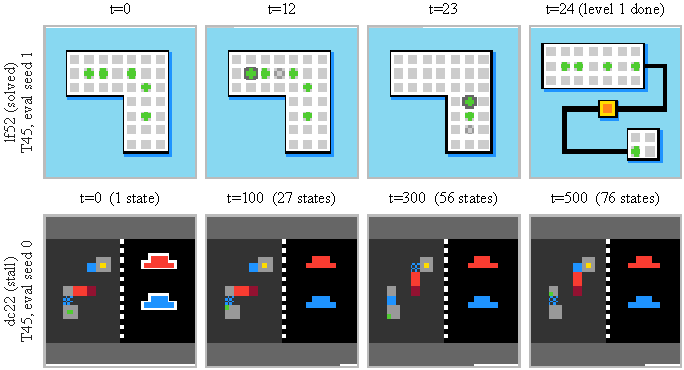
\includegraphics[width=0.62\textwidth]{figs/trajectories.pdf}
\caption{Recorded \Tn{45} frames. Top: lf52 level~1 solved in 24 actions (human 32); the next level's layout appears at $t{=}24$. Bottom: dc22 stall, with only 76 distinct ticker-masked states after 500 actions.}
\label{fig:traj}
\end{figure}
On move and mixed dev games every agent dies on a fixed per-life step budget (lives of $\sim$129/125/100/65 steps on ls20/dc22/ka59/lf52, identical for random, PPO and graph agents), so banning the last action before a death is wrong (\Tn{34}). On dc22 and ka59 the reachable states are exhausted within a few hundred actions (Fig.~\ref{fig:traj}), and relaxing pruning (\Tn{40}) finds no new ones. What is missing is a hypothesis about the goal, not more coverage. The LLM agent shows the same pattern: in Franzen's 100 public trajectories, stalls on later levels cost 43.9 points but inefficiency on solved levels only 2.6 \citep{skarin2026}.

\section{Discussion and limitations}
\textbf{Established.} (1) With sparse level rewards and 15 training games, neither DQN nor PPO learns transferable exploration, even with count, RND or effect shaping. Gains appear only with explicit per-game memory. (2) Pretrained effect predictors are at chance on unseen games, so ``what changes the frame'' must be learned online. (3) Hand-designed structure is very sample-efficient on the games it is tuned on and generalises poorly. \textbf{Uncertain.} Graph versions within $\approx$0.05 of each other are within seed noise (SD 0.04--0.09). Dev and held-out have 5 games each. Kaggle scores are single runs with $\pm$4 noise and unexplained failures. Compute is not matched to the LLM agent (an RTX PRO 6000 for 9\,h, vs.\ CPU seconds for ours). \textbf{Limitations.} 400k steps is small for deep RL \citep{henderson2018}, although 3--8 rewards per run suggests that the signal, not the budget, binds. The Kaggle checkpoint (training seed 0) was pre-registered, not chosen as the best seed.

\section{Conclusion}
For learning agents on ARC-AGI-3 the bottleneck is exploration within an unseen game, not value estimation or policy optimisation. Every gain we measured came from making per-game knowledge explicit and online, and those gains overfit a small dev set. A competitive score required a large pretrained model, whose single-run scores are too noisy to rank small modifications. Learning the explore-then-hypothesise loop itself, rather than hand-coding it, remains the open problem.

\paragraph{Generative-AI declaration.} Per the Wits academic-integrity policy: we used Claude and Claude Code (Anthropic) for planning, code, data analysis and drafting. We verified all code, numbers and text against our logs and take full responsibility for the content.
\paragraph{Member contributions.} [NAME 1]: [to be completed by the team]. [NAME 2]: [to be completed by the team].

\bibliography{refs}
\bibliographystyle{rlj}

\beginSupplementaryMaterials
\section{Hyperparameters, compute and all versions}
\begin{table}[h]
\centering\footnotesize
\caption{Compute. Training on one Kaggle T4 per seed (seeds in parallel); evaluation on Kaggle CPU, 1 thread per job, for 3 eval seeds $\times$ 5 dev games $\times$ 500 actions (per training seed). Test-time TD learning makes DQN evaluation $\sim$10$\times$ slower than PPO's. Total training: 10.45 T4-hours over 21 runs (incl.\ the \Tn{23} effect-model diagnostic).}
\label{tab:compute}
\begin{tabular}{@{}lrrrr@{}}
\toprule
Version & Train steps & Train h/seed (T4) & Eval s/train seed (CPU) & Train lv (s0/s1/s2) \\
\midrule
TEAM-10 DQN & 400{,}005 & 0.30--0.32 & 1{,}166 & 7/4/8 \\
TEAM-11 +novelty & 400{,}005 & 0.43--0.43 & 1{,}066 & 5/5/6 \\
TEAM-12 +effect mask & 400{,}005 & 0.49--0.50 & 1{,}350 & 4/6/4 \\
TEAM-20 PPO & 401{,}280 & 0.37--0.37 & 110 & 3/5/5 \\
TEAM-21 +RND & 401{,}280 & 0.45--0.46 & 68 & 5/7/6 \\
TEAM-22 +LSTM & 401{,}280 & 0.93--0.94 & 109 & 5/5/8 \\
TEAM-30 graph+online stats & 0 & -- & 89 (9 seeds) & -- \\
TEAM-37 +inverse actions & 0 (+T21 prior) & -- & 92 & -- \\
TEAM-45 component clicks & 0 (+T21 prior) & -- & 123 & -- \\
\bottomrule
\end{tabular}

\end{table}
\begin{table}[h]
\centering\scriptsize\setlength{\tabcolsep}{3pt}
\caption{Hyperparameters (identical across seeds; all learned versions: 400k steps on 15 games, episode cap 500; configs in \texttt{experiments/train/*/config.json}).}
\label{tab:hyper}
\begin{tabular}{@{}ll@{}}
\toprule
DQN (\Tn{10}--\Tn{12}) & replay 100k, batch 32, Adam $10^{-4}$, $\gamma$ 0.99, Huber, train every 4 steps, start 20k, hard target sync 10k,\\
 & $\epsilon$ 1.0$\to$0.05 over 200k; eval: $\epsilon$ 0.05, 1 TD update/action (batch 32, lr $10^{-4}$, target sync 100)\\
\Tn{11} / \Tn{12} & novelty $\beta=0.05$ (exact frame counts) / effect head BCE weight 1.0, mask threshold $p<0.1$\\
PPO (\Tn{20}--\Tn{22}) & MaskablePPO, $n_\text{steps}$ 128 $\times$ 15 envs, batch 240, 4 epochs, Adam $2.5\cdot10^{-4}$, $\gamma$ 0.99, GAE $\lambda$ 0.95, clip 0.2, entropy 0.01\\
\Tn{21} / \Tn{22} & RND coefficient 0.05, EMA($\alpha$=0.01)-normalised / + LSTM 256 (RecurrentPPO, masks as input channel)\\
Graph (\Tn{30}--\Tn{47}) & Beta(1,1)-Thompson effect stats; prior weight 0.3 (\Tn{31}+); prune after 3 failed tries; inverse pair after 2 undos, 0 counter-ex.;\\
 & ticker row: $\geq$10 changing steps, changes in $\geq$50\%, median $\leq$2 px, $\geq$3 actions; components $\leq$96 per state\\
\bottomrule
\end{tabular}
\end{table}
\begin{table}[h]
\centering\scriptsize\setlength{\tabcolsep}{2.5pt}
\caption{Every evaluated version (same columns as Table~\ref{tab:master}). G1 = graph exploration with the pretrained \Tn{12} effect head.}
\resizebox{\textwidth}{!}{\begin{tabular}{@{}llrrlrrr@{}}
\toprule
Ver. & Change & Dev score & Lv & Level~1 on dev: runs @ actions & Train & Held-out & Kaggle \\
\midrule
Rand. &  & 0.0004\,$\pm$\,0.0006 & 1 & lp85 1/3 @352 & 0.0111 & 0 & 0.02$^\dagger$ \\
\midrule
T10 & DQN & 0 & 0 & -- & -- & 0 & 0.00 \\
T10f & DQN frozen & 0 & 0 & -- & -- & -- & -- \\
T11 & +novelty & 0 & 0 & -- & -- & -- & 0.00 \\
T11f & frozen & 0 & 0 & -- & -- & -- & -- \\
T12 & +effect mask & 0.0044\,$\pm$\,0.0063 & 3 & lp85 3/9 @101--120 & 0.0002 & 0 & 0.00 \\
T12f & frozen & 0.0036\,$\pm$\,0.0033 & 6 & lp85 6/9 @116--307 & -- & -- & -- \\
T12a & mask only (no novelty) & 0.0028\,$\pm$\,0.0021 & 5 & lp85 5/9 @146--421 & -- & -- & -- \\
T12af & mask only, frozen & 0 & 0 & -- & -- & -- & -- \\
\midrule
T20 & PPO & 0.0004\,$\pm$\,0.0006 & 1 & lp85 1/9 @212 & -- & 0 & 0.00 \\
T21 & +RND & 0.0247\,$\pm$\,0.0317 & 5 & lp85 4/9 @124--489; ls20 1/9 @41 & 0.240 & 0.0005 & 0.05 \\
T22 & +LSTM & 0.0003\,$\pm$\,0.0004 & 1 & lp85 1/9 @241 & -- & 0 & -- \\
\midrule
G1 & graph + T12 effect head & 0.0013\,$\pm$\,0.0010 & 4 & lp85 4/9 @149--380 & -- & -- & -- \\
T30 & graph+online stats & 0.389\,$\pm$\,0.149 & 9 & lp85 9/9 @16--72 & 0.0578 & -- & -- \\
T31 & +PPO prior & 0.461\,$\pm$\,0.038 & 9 & lp85 9/9 @12--24 & -- & -- & -- \\
T32 & +ticker mask & 0.462\,$\pm$\,0.038 & 11 & lp85 9/9 @12--24; ls20 2/9 @413--416 & -- & -- & -- \\
T33 & +prune & 0.484\,$\pm$\,0.037 & 9 & lp85 9/9 @12--20 & -- & -- & -- \\
T34 & +timer deaths & 0.484\,$\pm$\,0.037 & 9 & lp85 9/9 @12--20 & -- & -- & -- \\
T35 & +click equivalence & 0.493\,$\pm$\,0.045 & 9 & lp85 9/9 @15--25 & -- & -- & -- \\
T35n & no prior & 0.471\,$\pm$\,0.073 & 15 & lp85 9/9 @15--21; ls20 6/9 @297--473 & 0.121 & -- & -- \\
T36 & prior on clicks & 0.494\,$\pm$\,0.045 & 15 & lp85 9/9 @15--25; ls20 6/9 @367--473 & -- & -- & -- \\
T37 & +inverse actions & 0.504\,$\pm$\,0.045 & 18 & lp85 9/9 @15--25; ls20 9/9 @128--287 & 0.0305 & 0.133 & 0.07 \\
T38 & patch stats & 0.124\,$\pm$\,0.081 & 18 & lp85 9/9 @17--220; ls20 9/9 @128--376 & -- & -- & -- \\
T39 & value frontier & 0.497\,$\pm$\,0.045 & 18 & lp85 9/9 @15--25; ls20 9/9 @205--421 & -- & -- & -- \\
T40 & relax when stuck & 0.503\,$\pm$\,0.045 & 18 & lp85 9/9 @15--25; ls20 9/9 @128--458 & -- & -- & -- \\
T41 & +object clicks & 0.470\,$\pm$\,0.088 & 26 & lf52 9/9 @34--95; lp85 9/9 @17--36; ls20 6/9 @240--413 & -- & -- & -- \\
T42 & small objects & 0.379\,$\pm$\,0.094 & 28 & ka59 1/9 @256; lf52 9/9 @35--99; lp85 9/9 @17--33; ls20 9/9 @128--287 & -- & -- & -- \\
T43 & objects as fallback & 0.545\,$\pm$\,0.079 & 27 & lf52 9/9 @52--349; lp85 9/9 @15--25; ls20 9/9 @128--287 & -- & -- & -- \\
T44 & object promotion & 0.568\,$\pm$\,0.063 & 27 & lf52 9/9 @46--295; lp85 9/9 @15--25; ls20 9/9 @128--287 & -- & -- & -- \\
T45 & component clicks & 0.791\,$\pm$\,0.087 & 27 & lf52 9/9 @24--56; lp85 9/9 @14--30; ls20 9/9 @128--287 & 0.0203 & 0.885 & -- \\
T45n & no prior & 0.667\,$\pm$\,0.222 & 28 & lf52 9/9 @23--59; lp85 9/9 @11--33; ls20 8/9 @128--374 & 0.0811 & 0.767 & -- \\
T46 & centres fallback & 0.791\,$\pm$\,0.087 & 27 & lf52 9/9 @24--56; lp85 9/9 @14--30; ls20 9/9 @128--287 & -- & -- & -- \\
T47 & size prior & 0.632\,$\pm$\,0.077 & 27 & lf52 9/9 @13--45; lp85 9/9 @16--49; ls20 9/9 @128--287 & -- & -- & -- \\
\bottomrule
\end{tabular}
}
\end{table}

\begin{figure}[h]
\centering
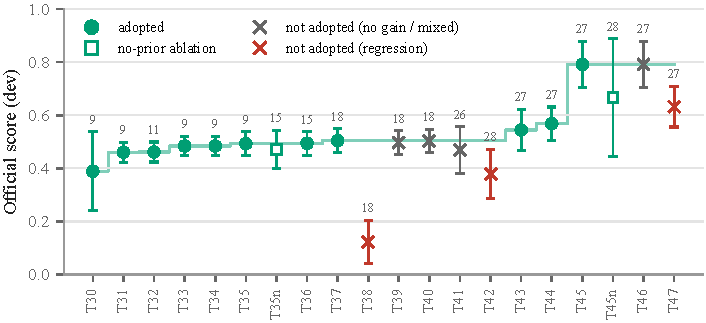
\includegraphics[width=\textwidth]{figs/graph_progression.pdf}
\caption{Graph-explorer progression on dev (mean $\pm$ SD over training seeds; numbers = levels). The line is the best adopted version so far. Red = regressions (\Tn{38} patch-keyed stats, \Tn{42} small objects only, \Tn{47} size prior).}
\label{fig:prog}
\end{figure}

\begin{figure}[h]
\centering
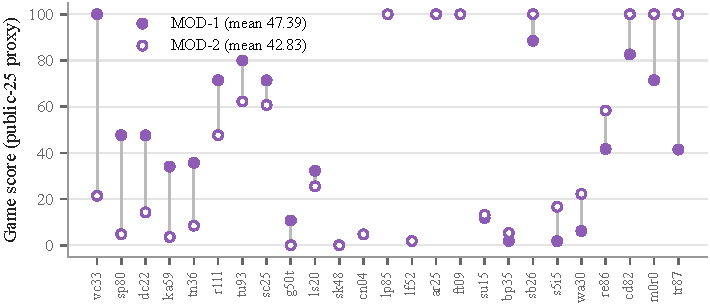
\includegraphics[width=\textwidth]{figs/proxy.pdf}
\caption{Matched one-pass proxy on the 25 public games (RTX PRO 6000, $\approx$2\,h each, launched together): MOD-1 47.39 vs.\ MOD-2 42.83. Per-game swings of up to 79 points in both directions show why one pass resolves only large effects.}
\end{figure}

\section{Kaggle submissions (evidence)}
All 16 submissions with IDs, script versions and output sizes are in \texttt{experiments/kaggle\_submissions.csv}. Nominated: submission \textbf{57556604}, notebook \texttt{thendonelufule/arc3-m2-modf-sub}, script version 359469291, public score \textbf{29.15}, 2026-10-23 09:42:37 UTC.

\end{document}
